\section{Component Architecture} \label{ComponentArchitecture}
In this section a class diagram will be designed to show the specifications of all complex components. This is done in order to create a flexible and understandable structure of the system.

\begin{figure}[H]
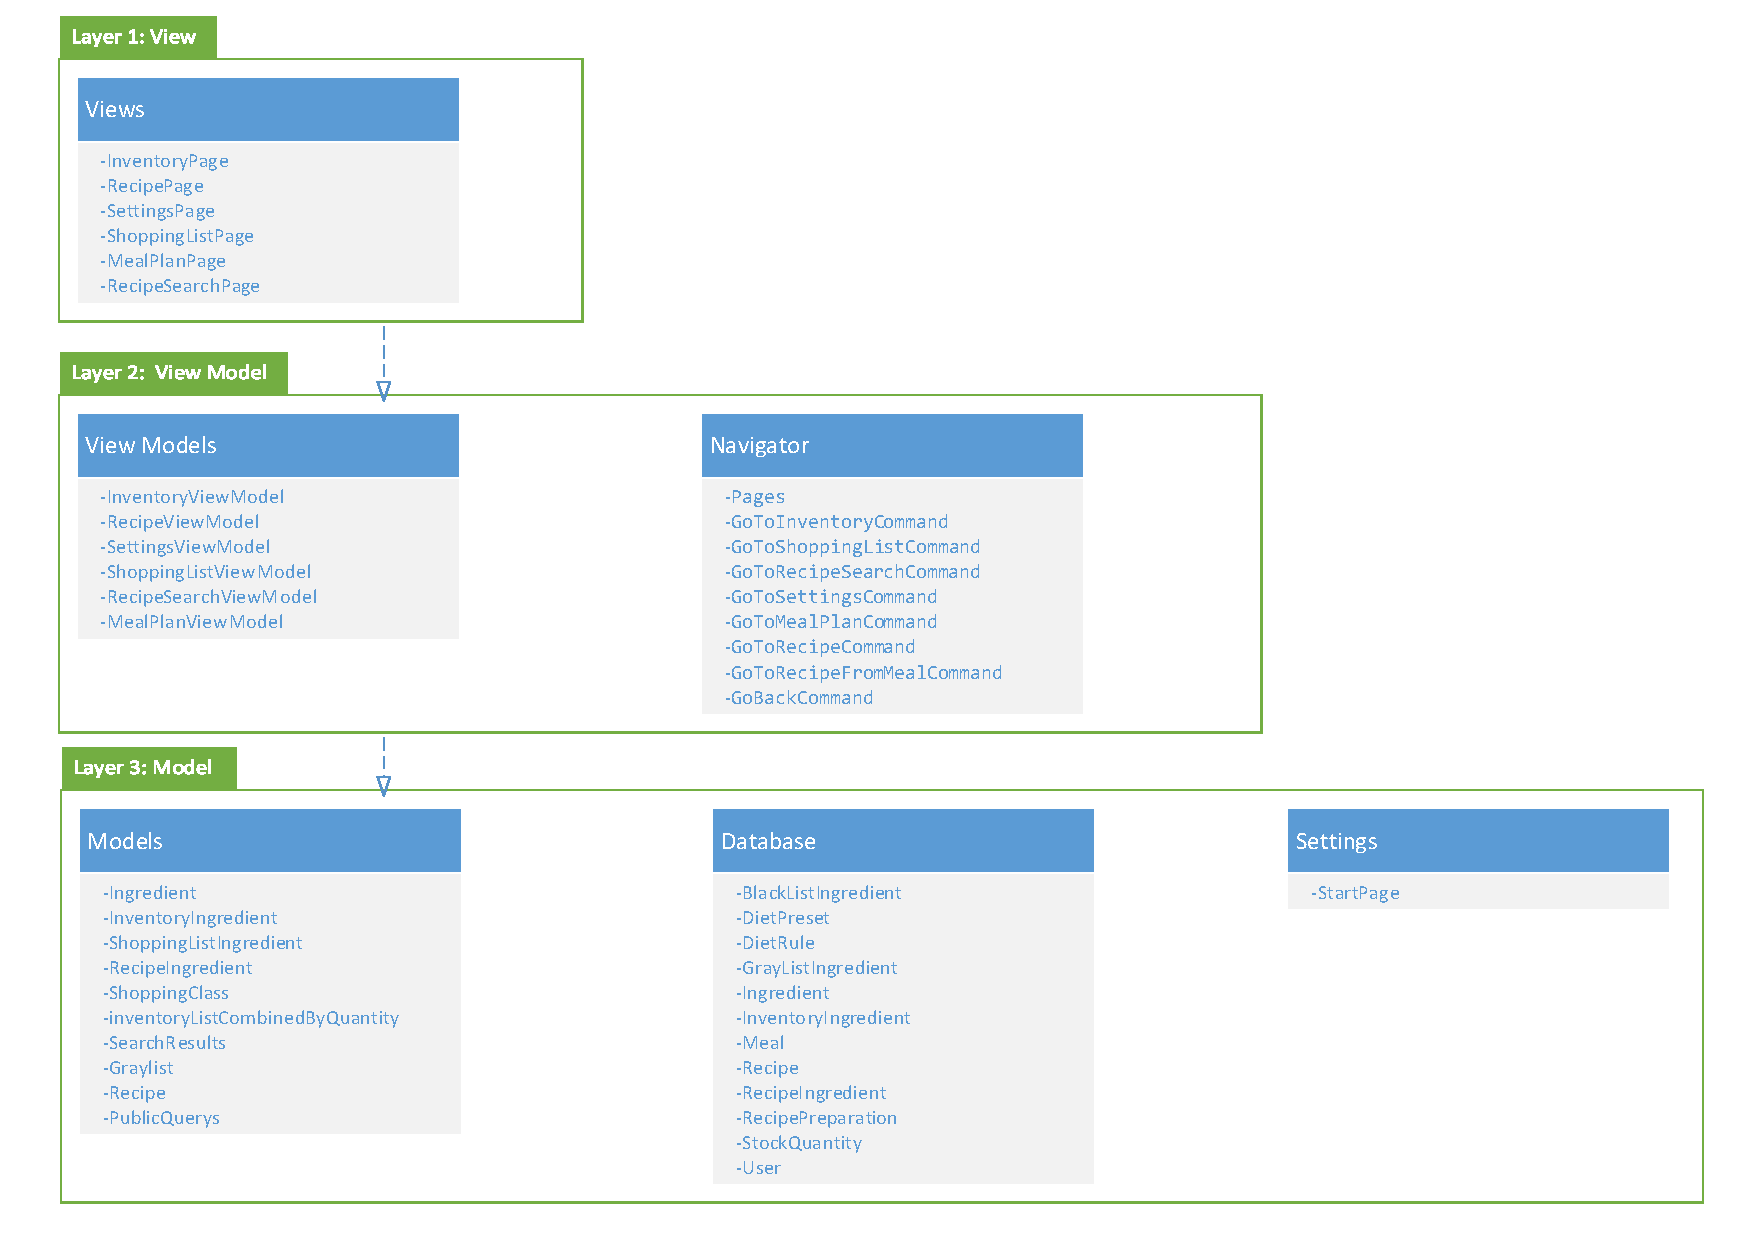
\includegraphics[width=\linewidth]{Grafik/FoodPlanner/ComponentDiagram}
\centering
\caption{Class layer diagram}
\label{LayerDiagram}
\end{figure}

\Cref{LayerDiagram} shows the class diagram for the components of the system. The pattern used is the MVVM pattern which is described in \Cref{MVVMSection}.

\paragraph{View}
The view component spans over the pages(windows) that are used to interact with the user. The responsibility of the View lies in that it shall send information to the View Model such that the user can interact with the system.

\paragraph{ViewModel}
The viewModel component spans over the classes that are associated with the pages in the view. The responsibility of the View Model is to give functionality to the model. The component uses the classes found in the Model. The viewModel also contains a Navigator which is used by the View and ViewModel itself and is responsible for letting the user navigate trough the different pages.

\paragraph{Model}
All the classes that are used in the system is going to be located in the Model component and is used directly by the ViewModel. The responsibility of the Model is to provide classes that can be used to manipulate data and synchronise such data with a database. The objects that can be created through the Model is used in the ViewModel. Another part of the Model is the settings. The settings are saved locally on the machine and is responsible for allowing some personal customization of the local processor.

There are an external standard component which is not shown on the diagram, the component is the Entity Framework which will be is used to simplify the data modification when it is saved or retrieved from/to the database, \Cref{EntityFrameworkSection} describes the framework in more detail.